%%%%%%%%%%%%%%%%%%%%%%%%%%%%%%%%%%%%%%%%%%%%%%%%%%%%%%%%%%%%%%%%%%%
%                                                                 %
%  GEANT manual in LaTeX form                                     %
%                                                                 %
%  Michel Goossens (for translation into LaTeX)                   %
%  Version 1.00                                                   %
%  Last Mod. Jan 24 1991  1300   MG + IB                          %
%                                                                 %
%%%%%%%%%%%%%%%%%%%%%%%%%%%%%%%%%%%%%%%%%%%%%%%%%%%%%%%%%%%%%%%%%%%
\Origin{R.Brun}
\Documentation{R.Brun, M.Maire}
\Version{Geant 3.16}\Routid{CONS199}
\Submitted{01.06.83}             \Revised{23.03.94}
\Makehead{The Material data structure JMATE}

\begin{figure}[hbt]
      \centering
      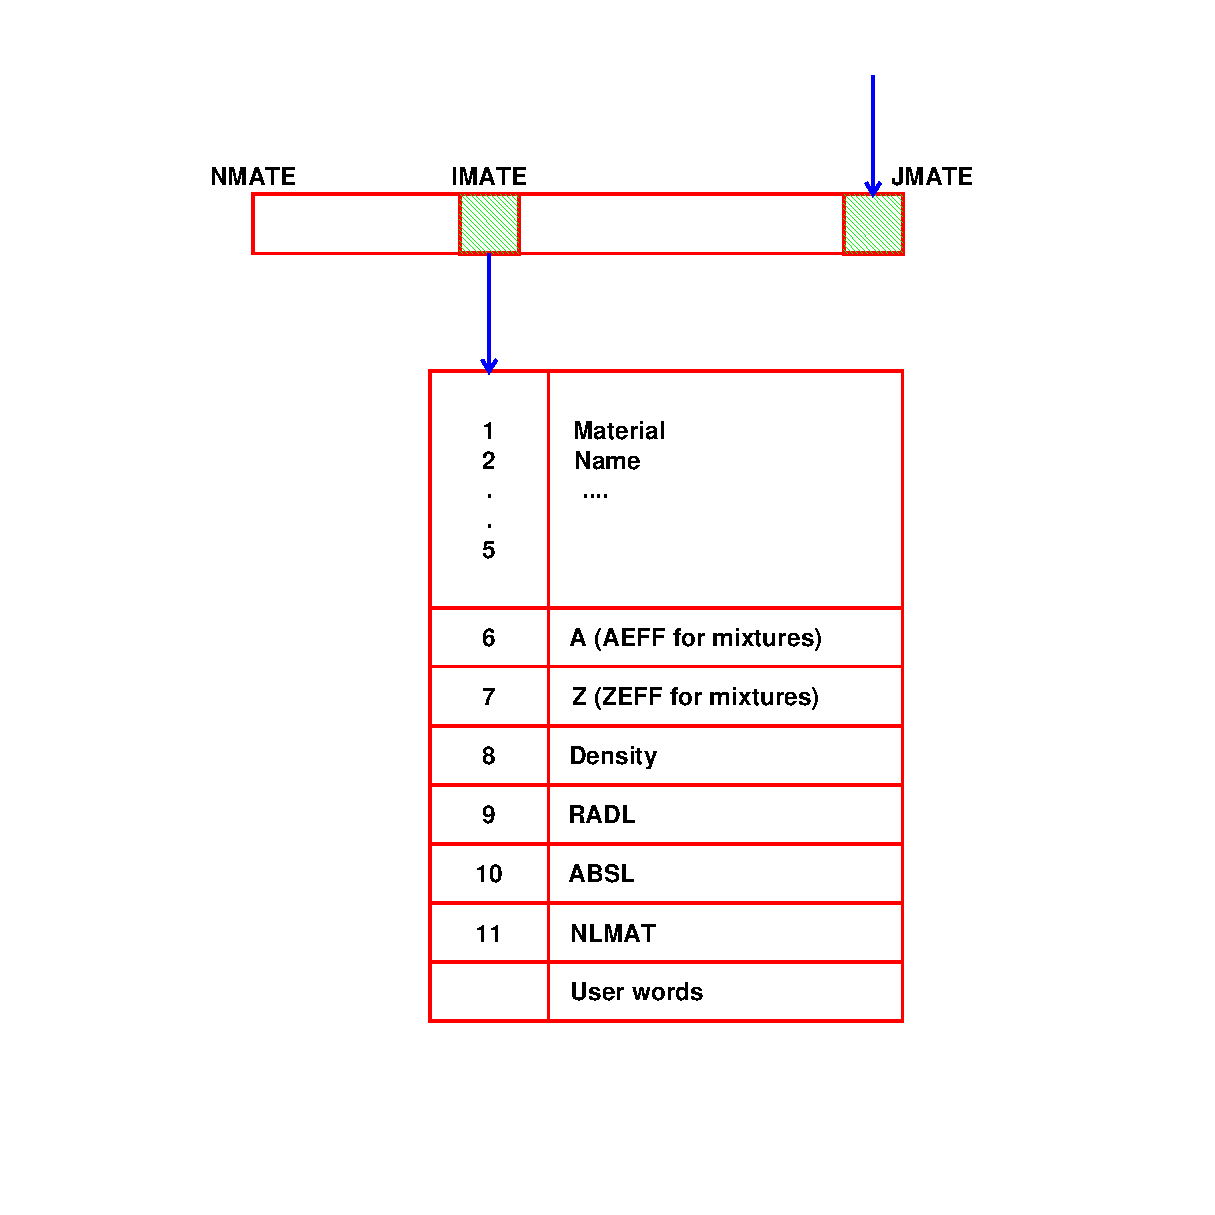
\epsfig{file=eps/cons199-1.eps,width=\linewidth}
      \caption{{\tt JMA = LQ(JMATE-IMATE)} pointer to material {\tt IMATE}}
      \label{cons199-1}
\end{figure}

When the subroutine GPHYSI is called at initialisation time the
following substructure is created for each material whose number
is refered to by any of the user defined tracking media.

\begin{figure}[p]
      \centering
      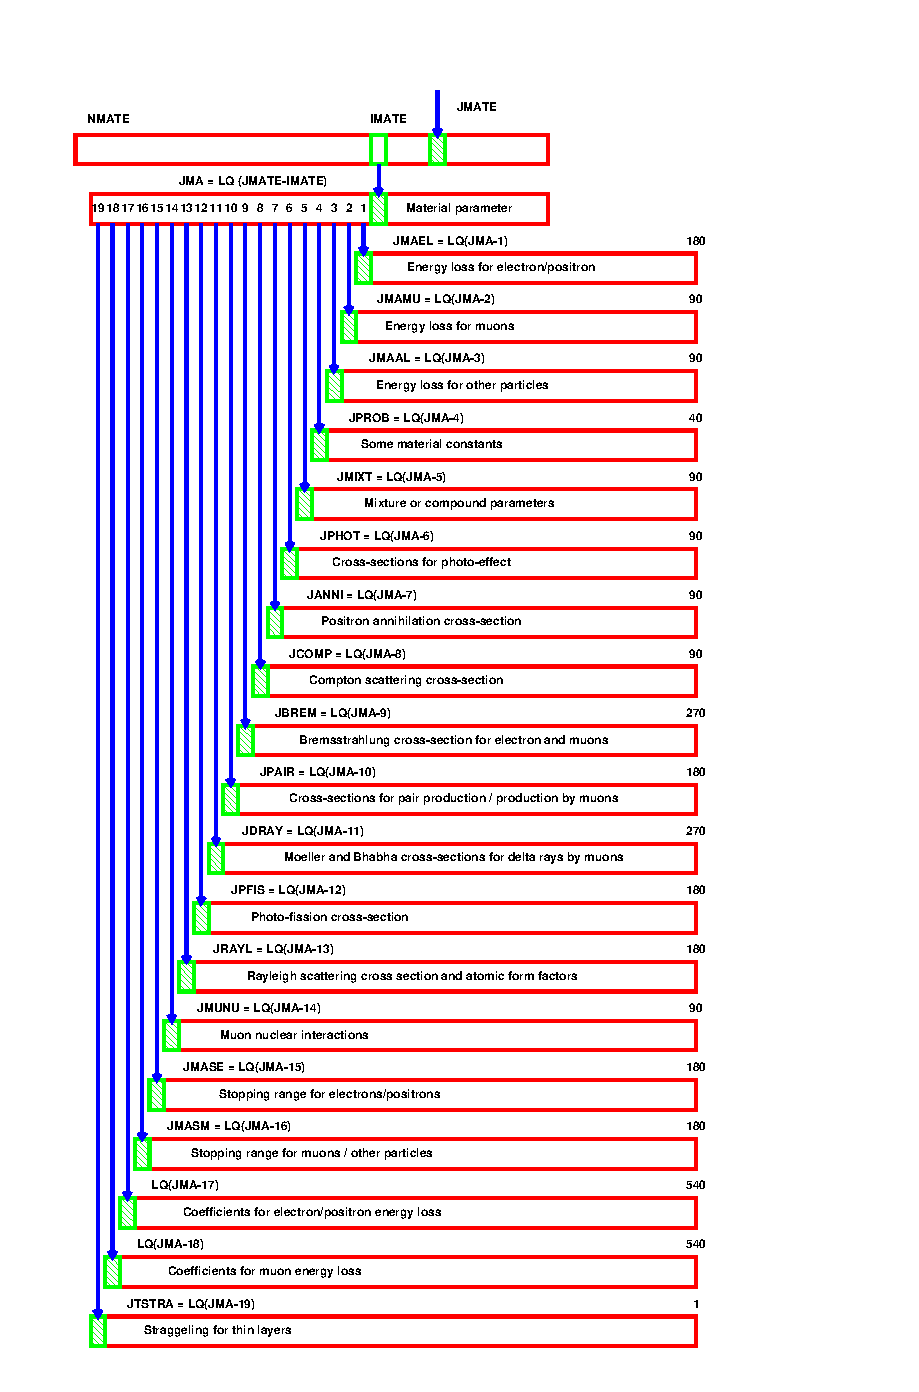
\epsfig{file=eps/cons199-2.eps,height=.95\textheight}
      \caption{Material data structure}
      \label{cons199-2}
\end{figure}

{\bf Note:}
The energy losses are stored in ${\rm GeV \: cm^{-1}}$. The inverse of
the macroscopic cross-section (i.e. the mean free path, in cm), is stored
instead of the cross-section, to speed up the calculation of the distance
to the next interaction point.
 
\section{Energy binning}
 
\begin{center}
\begin{tabular}{|c|l|l|}
\hline
IDECAD  &Bin number  &Energy range \\
& &IEKBIN    \\
\hline
 
1  &1 $\rightarrow$ 10  &10 KeV $\rightarrow$ 79.43 KeV          \\
2  &11 $\rightarrow$ 20  &100 KeV $\rightarrow$ 794.3 KeV       \\
3  &21 $\rightarrow$ 30  &1 MeV $\rightarrow$ 7.943 MeV           \\
4  &31 $\rightarrow$ 40  &10 MeV $\rightarrow$ 79.43 MeV         \\
5  &41 $\rightarrow$ 50  &100 MeV $\rightarrow$ 794.3 MeV       \\
6  &51 $\rightarrow$ 60  &1 GeV $\rightarrow$ 7.943 GeV           \\
7  &61 $\rightarrow$ 70  &10 GeV $\rightarrow$ 79.43 GeV         \\
8  &71 $\rightarrow$ 80  &100 GeV $\rightarrow$ 794.3 GeV       \\
9  &81 $\rightarrow$ 90  &1 TeV $\rightarrow$ 7.943 TeV           \\
\hline
\end{tabular}
\end{center}
 
The values of the bins are kept in the array ELOW(90) in /GCMULO/ :
 
\[
 \mbox{ELOW}(i) = 10 ^ { \frac{i-1}{10} - 5 } [ \mbox{GeV} ]
\]
 
\section{Energy loss for electrons and positrons}
 
Words 1 to 90, for electrons:  DE/DX = Ionisation (Moller) +brems.
 
Words 91 to 180, for positrons:  DE/DX = Ionisation (Bhabha) +brems.
[PHYS 330, 340].
 
\section{Energy loss for muons}
 
  DE/DX = Ionisation +brems. +Direct \Pep\Pem production +Nuclear interacti     on
[PHYS 430, 440, 450].
 
\section{Energy loss for other charged particles}
 
  DE/DX = Ionisation
 
The values are computed for a proton (mass Mp). For any other
particle with mass M and kinetic energy T,
one has to compute the equivalent proton kinetic energy as T*Mp/M
and look at the corresponding energy binning [PHYS 430].
 
\section{Some material constants}
 
Various constants which are material dependent and needed to compute the
cross-sections.
 
See routine GPROBI.
 
\section{Mixture and compound parameters}
 
Words 1 to 4*NLM  where  NLM is the number of mixture or compound
components [CONS110].
 
\section{Photo-electric effect. Muon nuclear interaction}
 
As the photo-electric effect vanishes at high energies
whereas the muon nuclear
interaction cross-section is null at low energies, the two effects are
stored within the same bank in order to save space.
 
From 10 KeV to 50 MeV : Photo-electric effect mean free path [PHYS 230]
From 1 GeV to 10 TeV : Muon nuclear interaction mean free path
[PHYS 460].
 
\section{Positron annihilation}
 
[PHYS 350].
 
\section{Compton scattering}
 
[PHYS 220].
 
\section{Bremsstrahlung for electrons and muons}
 
Words 1 to 90, mean free path for electrons [PHYS 340]
Words 91 to 180, mean free path for muons [PHYS 440].
 
\section{Pair production by gammas and muons}
 
Words 1 to 90, for gammas [PHYS 210].
Words 91 to 180, for muons [PHYS 450].
 
\section{Delta ray production by electrons and muons}
 
Words 1 to 90, for \Pem\Pem $\rightarrow$ \Pem\Pem [PHYS 330].
 
Words 91 to 180, for \Pep\Pem $\rightarrow$ \Pep\Pem [PHYS 330]
 
Words 181 to 270, for \Pem $\rightarrow$ \Pem [PHYS 430].
 
\section{Photo-fission}
 
Only for material with atomic number A>200 [PHYS 240].
%\end{document}
 
 
